\chapter{Opis projektnog zadatka}
		
\textit Cilj projekta je razviti online igricu Tanky. Igra je namijenjena za više igrača te je u potpunosti realizirana u web pregledniku. Svrha igrice je omogućiti zabavu i zanimaciju korisnicima te je namijenjena za svaki uzrast, međutim najviše je prilagođena mlađim te srednje starim korisnicima. Igra simulira rat oklopnih vozila te svaki igrač ima svoje vozilo koje se može kretati po mapi, a ta funkcionalnost izvodi se pomoću tipkovnice. Nadalje, igrači mogu ispaljivati projektile na protivnike kako bi ih eliminirali. Igrač projektil usmjeruje pomoću miša te ga klikom na lijevi gumb ispaljuje. Pogotkom se pogođenom igraču smanjuje život te ukoliko dođe do nule eliminira ga se iz igrice, a igraču koji ga je pogodio se evidentiraju bodovi. Igrači se natječu u rundama ograničenog trajanja i igrač s najviše ostvarenih bodova pobjeđuje.

Ulaskom u igricu korisniku se prikazuje početni izbornik koji je prikazan slikom 2.1. Korisnik se može pridružiti kao registrirani ili kao anonimni korisnik. 

\begin{figure}[h]
	\centering
	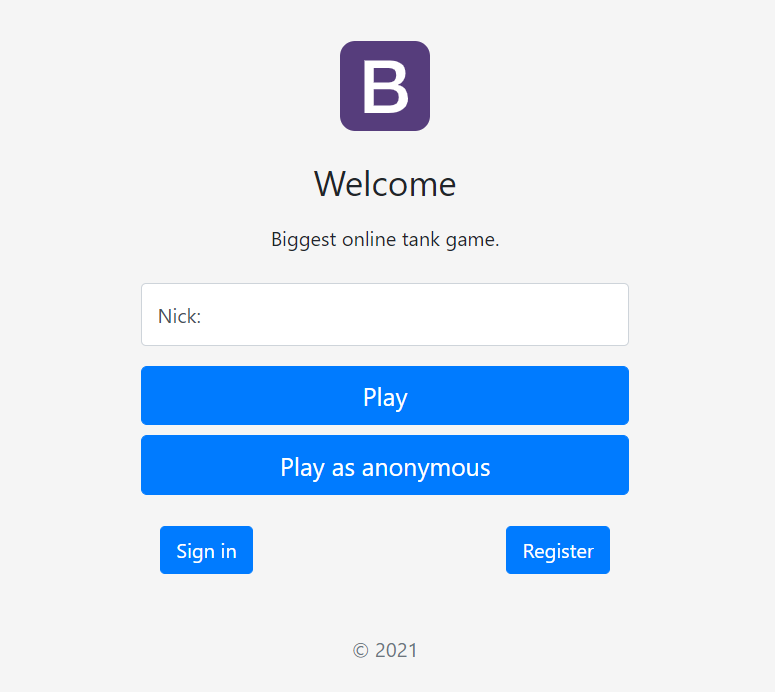
\includegraphics[width=7cm,height=7cm]{startMenu}
	\caption{Početni izbornik}
	\label{fig:opis}
\end{figure}

Prilikom registracije korisnik mora upisati e-mail adresu i lozinku koju će onda koristiti svaki sljedeći put prilikom prijave. 
Prije pokretanja same igre korisnik upisuje nadimak koji će se koristiti za prikaz rezultata trenutno aktivne runde u gornjem desnom kutu ekrana. Nakon pokretanja korisnik je automatski pozicioniran na mapu s ostalim igračima te igra započinje. Na mapama se nalaze razne prepreke i zakloni gdje se igrač može skloniti od protivnika. Također, igrica automatski spaja igrače slične jačine (broja bodova) u iste igre tako da igra bude što zanimljivija i ravnopravnija.

Registriranim korisnicima se prati broj rundi u kojima su sudjelovali te prikazuje statistika pobjeda u izborniku „Moj račun“. Nadalje, registrirani korisnici imaju mogućnost promjene izgleda njihovog oklopnog vozila u tom istom izborniku, klikom na željeni izgled među dostupnima. Izgledi se otključavaju ovisno o postignutim bodovima igrača. Korisnički izbornik nudi i mogućnost promjene zaporke, resetiranja statistike, brisanja računa i pregled statistike drugih registriranih korisnika pretraživanje po nadimku.
Unutar same web aplikacije postoji uloga administratora. Administrator ima posebno sučelje unutar kojeg ima niz opcija. Jedna od opcija je određivanje liste mapa koje su trenutno aktivne unutar same igre od ponuđenih. Daljnje opcije su pretraga korisnika po nadimku, prikaz statistike, zabranjivanje korisnicima pristup igri te uklanjanje korisnika.
Trenutno aktivna runda u donjem desnom kutu ima prozor za razgovor. Koristeći taj prozor igrači mogu izmjenjivati poruke. 

Ideju i motivaciju za igru pronašli smo u sličnim popularnim igrama namijenjenim za više igrača. Jedan od primjera je AZ Tank Game sa slike 2.2, igra s vrlo sličnom tematikom međutim namijenjena samo za igru 1 na 1. \\

\begin{figure}[h]
	\centering
	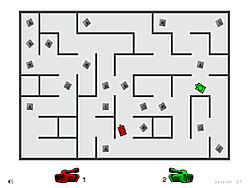
\includegraphics[width=7cm,height=7cm]{AZtankGame}
	\caption{AZ Tank Game}
	\label{fig:opis}
\end{figure}



\textit Također, igre poput Agar.io i Slither.io koje su tematski različite, ali idejno iste kao Tanky, čija smo rješenja i implementaciju proučavali kako bi dobili ideje za razvoj naše igrice.

Na slici 2.3 prikazana je igrica Slither.io koja je također namijenjena za više korisnika koji igraju jedan protiv drugog. Međutim za razliku od Tanky-a gdje je cilj pogoditi protivnika projektilom ovdje igrači pokušaju natjerati protivnike da se zabiju u tijelo njihove „zmije“ te ih tako eliminirati iz igre.

\begin{figure}[h]
	\centering
	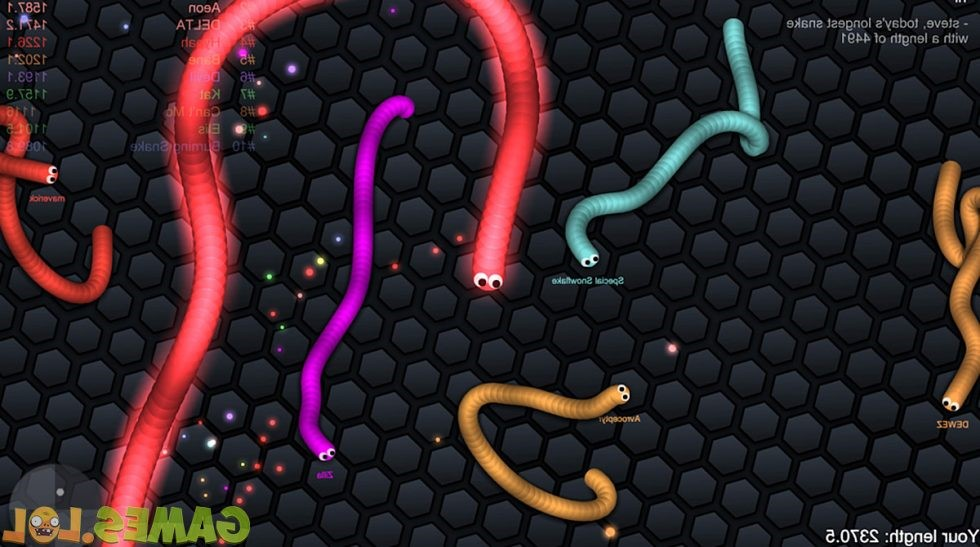
\includegraphics[width=7cm,height=7cm]{ioExample}
	\caption{Slither.io}
	\label{fig:opis}
\end{figure}

Problematizacija i opseg zadatka svodi se na razvoj back-end i front-end dijelova aplikacije u skladu s objektno orijentiranom paradigmom te na osmišljanje i izradu dizajna pojedinih elemenata. Za front-end implementaciju koristili smo HTML, CSS i JavaScript. Za back-end razvoj koristili smo Javascript, SQL te sustav za upravljanje bazama PostgreSQL u kojem smo postavili bazu podataka.

Projekt je sklon brojnim nadogradnjama koje je moguće provesti. Jedna od njih je uvođenje mogućnosti formiranja timova unutar igre. Tim bi se sastojao od minimalno dva igrača. Kreiranje runde bilo bi moguće samo za timove u kojima je isti broj igrača. Također, jedna od nadogradnji je uvođenje lige. U ligu bi mogli ući samo igrači koji su ostvarili potreban kvalifikacijski broj bodova. Liga bi se održavala 3 dana u tjednu. Kvalificirani igrač odigrao bi određen broj rundi i bio plasiran prema svom dostignuću, a isto tako i nagrađen poboljšanjima tenka.\\
 		
	